% 原印刷109--119页／PDF物理135--145.
\subsection{讨论}\label{sec:3.3}
\subsubsection{不同范数与更一般的凸成本}\label{sec:3.3.1}\index{C029@凸传输成本（convex transport costs）|hyperpage}
细心的读者会注意到，\autoref{sec:3.1}中关于距离成本函数的证明，专门针对欧氏范数诱导的距离. 从Monge原问题出发，沿着Sudakov\cite{b290}的证明策略（其中一个缺口后来由Ambrosio在\cite{b8,b10}中解决，但该策略原本是为了处理任意范数），不同范数的情形在近年得到广泛研究. 注意，一致凸范数（即其范数平方的Hessian矩阵以下方某个正定矩阵为界）的情形，与欧氏情形最接近，可以类似处理.

最早的推广之一，是Ambrosio、Kirchheim与Pratelli研究的晶体范数\cite{b14}，即单位球为凸多面体的范数. 可以猜想，面数有限会让任务更容易，但这仍需要大量逼近工作. 事实上，若使用对偶性，Kantorovich势的梯度$\nabla u(x)$不足以确定$(x,y)\in\operatorname{spt}(\gamma)$的位移$y-x$的方向，因为晶体范数在同一个面的所有点上具有相同梯度（而不仅仅是在同一射线上的点上，后者是欧氏范数及其他严格凸范数的情形）. 为处理这一问题，\cite{b14}发展了一种双重逼近策略：将$\|z\|$替换为类似$\|z\|+\varepsilon|z|+\varepsilon^2|z|^2$的表达式，其中$\|z\|$为所考虑的范数，$|z|$是为选定方向而加入的欧氏范数，再加入它的平方以得到严格凸性和每条射线上的单调性（恰如\autoref{sec:3.1}所见）. 由此，作者证明了任意维数中晶体范数、以及$\mathbb R^2$中任意范数的最优映射存在性.

后来，推广到其他范数的道路也被打开. 主要工具仍是次级变分问题，因为对于范数成本，并非所有最优方案都来自映射，必须选取一个特殊方案. 次级变分问题的困难在于，它们对应的新成本$c$不处处有限，因而无法对次级问题使用对偶性. 事实上，\hyperref[obj:1.42]{命题1.42}证明，对所有下半连续成本，原问题与对偶问题的值相等，但不保证对偶最优解存在；存在性通常或者用Ascoli--Arzelà论证保证，或者通过要求成本有限的\autoref{obj:1.37}保证. 因而发展出一些避免对偶性、集中于$c$-循环单调性的方法. 这些方法最早出现在\cite{b122}，针对另一个问题（$L^\infty$情形）：它对应于\autoref{sec:3.2}中介绍的想法，即寻找方案所集中集合的密度点. \phantomsection\label{idx:i58-p110}\index{E058@最优映射的存在性（existence of an optimal map）|hyperpage}
随后，Champion与De Pascale用相同工具，先证明了任意严格凸范数的最优映射存在性（\cite{b119}；几乎同时，Caravenna在\cite{b103}中以不同方式得到同一结果），再在\cite{b120}中证明了一般范数的情形. 后一个结果更难，需要额外的逼近工具，其灵感来自\cite{b273}，特别是像\autoref{sec:3.1.5}中那样，通过原子边缘测度逼近来选取一个特殊最优方案.

但最优传输的发展不只考察范数. 人们还对不同成本函数做了许多研究（流形上的距离或距离平方、$\mathbb R^d$中存在障碍时的测地距离，等等）. 本书倾向于保持在欧氏情形，本节只考虑$c(x,y)=h(x-y)$、$h$凸的成本. 即便这一情形，也远未完全理解. 在与Carlier、De Pascale合著的论文\cite{b113}中，我们提出一个按照成本函数$h$的“面”来分解的一般策略（它是直接的）.

分解基于以下步骤：
\begin{itemize}
\item 考虑最优方案$\gamma$，考察\autoref{sec:1.3}那样的最优性条件. 对所有$(x_0,y_0)\in\operatorname{spt}(\gamma)$，若$x_0$为势$\varphi$的可微点（记作$x_0\in\operatorname{Diff}(\varphi)$），则$\nabla\varphi(x_0)\in\partial h(x_0-y_0)$；这等价于
\begin{equation}\label{eq:3.6}
x_0-y_0\in\partial h^*(\nabla\varphi(x_0)).
\end{equation}
定义
\[
\mathscr F_h:=\{\partial h^*(p):p\in\mathbb R^d\},
\]
即$h^*$的次微分多值映射的所有可能取值所成的集合. 这些取值是$h$在其上仿射的凸集，将称为$h$的\emph{面}. 假设$\mu\ll\mathscr L^d$且$h$为Lipschitz函数，从而$\varphi$也为Lipschitz函数，就能保证$\varphi$在$\mu$-几乎处处可微. 由\eqref{eq:3.6}，对于每个固定的$x$，所有满足$(x,y)$属于某个最优传输方案支集的点$y$，都使差$x-y$属于$h$的同一个面. 经典地，当这些面都是单点（即$h^*$可微，等价于$h$严格凸）时，就用这种方法得到传输映射，因为每个$x$仅容许一个$y$.

\eqref{eq:3.6}还可将点$x$如下分类. 对每个$K\in\mathscr F_h$，定义
\[
X_K:=\{x\in\operatorname{Diff}(\varphi):\partial h^*(\nabla\varphi(x))=K\}.
\]
于是按$x\in X_K$这一标准，可将$\gamma$分成若干子方案$\gamma_K$. 当$K$遍历所有可能的面时，这一分解覆盖$\gamma$-几乎所有点对$(x,y)$. 此外，若$(x,y)\in\operatorname{spt}(\gamma)$且$x\in\operatorname{Diff}(\varphi)$，则$x\in X_K$蕴含$x-y\in K$.

若$\mathscr F_h$有限或可数，定义
\[
\gamma_K:=\gamma_{|X_K\times\mathbb R^d}.
\]
这时，$\gamma_K$的边缘测度$\mu_K,\nu_K$（即它分别经映射$\pi_x,\pi_y$得到的像）分别为$\mu,\nu$的子测度. 特别地，$\mu_K$从$\mu$继承绝对连续性. 这对证明传输映射存在往往很有用.

若$\mathscr F_h$不可数，在某些情形仍可考虑集合$\mathscr F_h^{\mathrm{multi}}:=\{K\in\mathscr F_h:K\text{ 不是单点}\}$，借助可数分解处理. 若$\mathscr F_h^{\mathrm{multi}}$可数，可以分离出$\partial h^*(\nabla(\varphi(x)))$为单点的那些$x$（那里已经存在传输），只对$K\in\mathscr F_h^{\mathrm{multi}}$进行分解.

\item 这一分解把传输问题化为如下类型的传输问题的叠加：
\[
\min\left\{\int h(x-y)\,d\gamma(x,y):\gamma\in\Pi(\mu_K,\nu_K),\ \operatorname{spt}(\gamma)\subset\{x-y\in K\}\right\}.
\]
优点在于，成本$c$限制在$K$上后更容易研究. 若$K$是$h$的一个面，则$h$在$K$上仿射，这时传输成本不再依赖于传输方案.

\item 问题化为寻找把$\mu_K$送到$\nu_K$且满足约束$x-\mathrm T(x)\in K$的传输映射，并且事先知道，存在满足同样约束的传输方案.

在某些情形（例如$K$为内部包含$0$的紧凸集），这一问题可以化为$L^\infty$传输问题. 事实上，若以$\|\cdot\|_K$表示满足$K=\{x:\|x\|_K\le1\}$的（类似规范泛函的）“范数”，则
\begin{equation}\label{eq:3.7}
\min\left\{\max\{\|x-y\|_K:(x,y)\in\operatorname{spt}(\gamma)\}:\gamma\in\Pi(\mu,\nu)\right\}\le1,
\end{equation}
问题是：如果把可行集限制为传输映射，即从Kantorovich转到Monge，同一不等式是否仍成立？若\eqref{eq:3.7}的某个解由传输映射$\mathrm T$诱导，答案就是肯定的. 当$K=B(0,1)$时，这正是\autoref{sec:3.2}所介绍的结果；它最早在\cite{b122}中用不同策略证明（不用次级变分问题选取极小元，而是在$p\to\infty$时选取$L^p$范数极小元的极限）. 还要注意，这一问题在一维很容易，单调传输解出所有$L^p$问题，因而也解出$L^\infty$问题（而且不要求测度绝对连续，只需无原子）.
\end{itemize}

注意，面数可数这一假设限制很强，主要是为了保证$\mu_K$绝对连续，而无需测度分解论证（后者可能导致至少与Sudakov面对的困难一样难、与Sudakov面对的困难一样难的问题；另见\cite{b104}）. 不过，晶体范数是可用有限分解处理的一个有意思的例子. 这时成本$h$的面是多面锥，但若两个测度支集有界，可以假设它们是紧凸多面体. 由上述讨论，这意味着可进行有限分解，把问题化为单位球为多面体（即锥的面）的范数的若干$L^\infty$极小化问题. 特别地，如果能解出其他晶体范数的$L^\infty$最优传输问题，就能解决晶体范数的$L^1$问题.

于是，像\autoref{sec:3.2}那样解决$L^\infty$问题，并把单位球约束$|x-y|\le1$换成更一般的约束$x-y\in C$，就很有意义，其中$C$为一般凸集，例如多面体. \cite{b197}通过极小化二次成本
\[
c(x,y)=\begin{cases}|x-y|^2,&x-y\in C,\\+\infty,&\text{否则},\end{cases}
\]
研究这一问题，它同样形如$c(x,y)=h(x-y)$，其中$h$严格凸（但并非实值）. 当$\mu$绝对连续，且$C$或者严格凸、或者具有可数个面时，可以证明最优映射存在（更确切地说，该问题每个最优$\gamma$都由映射诱导）. 通过改写\autoref{sec:3.2}的论证，并证明如果$(x_0,y_0)$和$(x_0,y_1)$属于$\operatorname{spt}(\gamma)$（从而$y_0-x_0,y_1-x_0\in C$），则中点$\frac12(y_0+y_1)-x_0$不可能位于$C$的内部，就能做到这一点. 若$C$严格凸，这证明$y_0=y_1$. 若不严格凸，这证明$y_0-x_0$与$y_1-x_0$在$C$的同一个面上，从而可以降维并进行归纳.

特别地，这一论证适用于多面体及$\mathbb R^2$中的任意凸集（因为$\partial C$至多包含可数条线段），并给出\cite{b14}结果的另一证明.

关于最后一个结果已有许多推广：Bertrand与Puel\cite{b52}研究了“相对论”成本$h(z):=1-\sqrt{1-|z|^2}$，它自然带有约束$|z|\le1$，且为严格凸函数（但并非处处有限，因为约束意味着单位球外$h(z)=+\infty$）. 他们将\cite{b122,b197}的论证推广到严格凸函数$h$与严格凸约束$C$的情形，证明了最优映射存在（由此看来，推广到可数个面的情形也应可行）.

最后，Chen、Jiang与Yang结合\cite{b197}和\cite{b120}的论证，在对$C$的通常假设（严格凸或面数可数）下，得到成本函数
\[
c(x,y)=\begin{cases}|x-y|,&x-y\in C,\\+\infty,&\text{否则}\end{cases}
\]
的存在性. 这些结果见\cite{b123,b124}，首次同时处理了缺少严格凸性和无穷值.

这些接连的改进为一个明显的猜想铺平了道路：对偶性、变分逼近与密度点技巧的结合，最终或可在非常一般的情形证明最优传输映射存在：
\begin{problem*}[每个凸成本的存在性]
假设$\mu\ll\mathscr L^d$，成本$c(x,y)$形如$h(x-y)$，其中$h:\mathbb R^d\to\mathbb R\cup\{+\infty\}$凸；证明存在最优映射.
\end{problem*}
这一问题一直开放到本书最后成稿阶段，当时Bardelloni与Bianchini的论文\cite{b26}出现，证明了一个测度分解结果，它蕴含的正是这一陈述，至少在$h$有限但不严格凸的情形如此.

\subsubsection[凹成本]{凹成本：$L^p$，$0<p<1$}\label{sec:3.3.2}
另一类在应用中十分合理的传输成本，并非欧氏距离的凸函数，而是凹成本\footnote{这里指关于距离$|x-y|$为凹函数的成本，不是\autoref{obj:2.12}中考虑的关于位移$x-y$为凹函数的成本.}，更确切地说，$c(x,y)=\ell(|x-y|)$，其中$\ell:\mathbb R_+\to\mathbb R_+$严格凹且递增\footnote{不会每次都显式说明，但这还蕴含$\ell$严格递增.}. 从经济学和建模角度，这是最自然的选择：移动质量的成本，随着距离增加，按比例算会更低；多数交通方式的票价或费用（铁路、高速公路通行费、航空等等）都能说明这一点. \phantomsection\label{idx:i145-p114}\index{S145@次可加性（sub-additivity）|hyperpage}
这些成本全都次可加. 许多实际情况下，把两份质量各移动距离$d$，比让一份移动$2d$、另一份留在原地更昂贵. 具有这些性质的典型例子是幂成本$|x-y|^\alpha$，$\alpha<1$.

\phantomsection\label{idx:i44-p114}\index{D044@距离成本（distance costs）|hyperpage}
注意，这些成本都满足三角不等式，因而是$\mathbb R^d$上的距离. 此外，在严格凹性假设下，它们满足严格三角不等式. 后一事实意味着，$\mu$与$\nu$的共同质量必须留在原地，这最早由\cite{b176}指出.

\begin{theorem}\label{obj:3.25}
设$\gamma$是成本$c(x,y)=\ell(|x-y|)$的最优传输方案，其中$\ell:\mathbb R_+\to\mathbb R_+$严格凹、递增，且$\ell(0)=0$. 写成$\gamma=\gamma_D+\gamma_O$，其中$\gamma_D$是$\gamma$在对角线$D=\{(x,x):x\in\Omega\}$上的限制，$\gamma_O$是对角线之外的部分，即在$D^c=(\Omega\times\Omega)\setminus D$上的限制. 则这一分解满足：$(\pi_x)_\#\gamma_O$与$(\pi_y)_\#\gamma_O$互相奇异.
\end{theorem}
\begin{proof}
显然$\gamma_O$集中于$\operatorname{spt}(\gamma)\setminus D$，从而$(\pi_x)_\#\gamma_O$集中于$\pi_x(\operatorname{spt}(\gamma)\setminus D)$，$(\pi_y)_\#\gamma_O$集中于$\pi_y(\operatorname{spt}(\gamma)\setminus D)$. 断言这两个集合互不相交. 事实上，反设有共同点$z$属于二者. 根据定义，存在$y$使$(z,y)\in\operatorname{spt}(\gamma)\setminus D$，并存在$x$使$(x,z)\in\operatorname{spt}(\gamma)\setminus D$. 因而可以对$(x,z)$与$(z,y)$应用$c$-循环单调性，得到
\begin{equation*}
\begin{aligned}
\ell(|x-z|)+\ell(|z-y|)&\le\ell(|x-y|)+\ell(|z-z|)\\
&=\ell(|x-y|)<\ell(|x-z|)+\ell(|z-y|),
\end{aligned}
\end{equation*}
最后的严格不等式给出矛盾.
\end{proof}

这为构造最优方案$\gamma$给出第一条限制：考察$\mu,\nu$，取共同部分$\mu\wedge\nu$并让它留在原地，将它从其余部分中减去，再在没有共同质量的两个剩余部分之间构造最优传输. 注意，当成本$c$关于欧氏距离线性时，共同质量\emph{可以}留在原地，却不被迫如此（想想搬书例子）；相反，若成本是欧氏距离的严格凸函数，共同质量一般\emph{不}留在原地（在前例中，$c(x,y)=|x-y|^p$、$p>1$时，只有平移最优）. \phantomsection\label{idx:i112-p115}\index{N112@最优映射的不存在性（non-existence of optimal maps）|hyperpage}
共同质量留在原地，意味着一般不存在最优映射$\mathrm T$：只要存在集合$A$使$\mu(A)>(\mu\wedge\nu)(A)=\nu(A)>0$，则$A$中几乎每点都必须有两个像：它自己，以及$A$外的另一点.

\begin{figure}[htbp]\centering
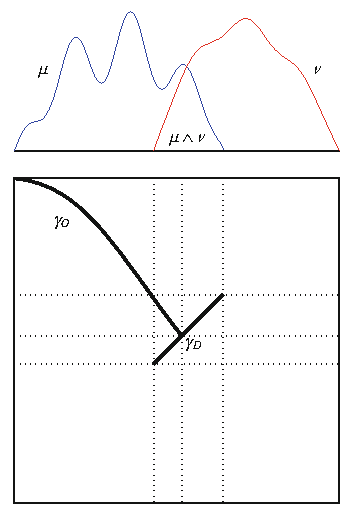
\includegraphics[width=.54\textwidth]{assets/ch03-fig-3-5.pdf}
\caption{有共同质量时，一维情形中的最优方案.}\label{fig:3.5}
\end{figure}

\autoref{fig:3.5}展示一维的典型情况；由\autoref{obj:2.12}，去除共同质量后的传输映射递减. 注意，对于这类一维“凹”成本，最优传输映射的精确结构遵循某种分层构造，最早由\cite{b230}研究，随后在\cite{b141}中用于数值目的.

这提示研究$\mu,\nu$互相奇异的情形，而能得到的最好结果，是证明这时存在最优映射. 特别地，这使我们能够避开函数$(x,y)\mapsto\ell(|x-y|)$在对角线$\{x=y\}$上的奇性（考虑$|x-y|^\alpha$），因为当两个测度没有共同质量时，几乎没有点$x$被传输到$y=x$.

不过，利用这一事实仍需谨慎. 最简单的情形是$\mu,\nu$支集互不相交，这时$|x-y|$有正下界，因而可以远离奇点. 但$\operatorname{spt}(\mu)\cap\operatorname{spt}(\nu)=\varnothing$限制过强，因为即便$\mu,\nu$具有光滑密度$f,g$，减去共同质量后，两个支集仍可能在$\{f=g\}$区域相遇.

Gangbo与McCann的经典论文\cite{b176}解决了这一问题，它也是最早的最优传输论文之一. 文中使用稍弱的假设$\mu(\operatorname{spt}(\nu))=0$. 这一假设涵盖上面两个连续密度的例子，但不涵盖许多其他情形. 例如$\mu$为有界区域$\Omega$上的Lebesgue测度，而$\nu$是在每个有理点都有原子的原子测度；也可以构造另外的例子，使用支集为全空间、却分别集中于互不相交的集合$A$与$\Omega\setminus A$上的绝对连续测度（见\autoref{ex:20}）. 本节将说明，当$\mu,\nu$互相奇异且$\mu\ll\mathscr L^d$时，怎样证明传输映射存在.

我们将证明如下结果.
\begin{theorem}\label{obj:3.26}
设$\mu,\nu$是$\mathbb R^d$上互相奇异的两个概率测度，且$\mu\ll\mathscr L^d$；取成本$c(x,y)=\ell(|x-y|)$，其中$\ell:\mathbb R_+\to\mathbb R_+$严格凹、在$]0,+\infty[$上为$C^1$且递增. 则存在唯一最优传输方案$\gamma$，且它由传输映射诱导.
\end{theorem}
\begin{proof}
使用\autoref{sec:1}中针对形如$c(x,y)=h(x-y)$的成本介绍的标准方法. 特别地，存在一个Kantorovich势$\varphi$，使得若$(x_0,y_0)\in\operatorname{spt}(\gamma)$，则
\begin{equation}\label{eq:3.8}
x_0-y_0=(\nabla h)^{-1}(\nabla\varphi(x_0)).
\end{equation}
这使我们可以把$y_0$表示为$x_0$的函数，从而证明$\operatorname{spt}(\gamma)$中只有一个点$(x_0,y)$，所以$\gamma$来自传输$\mathrm T(x)=x-(\nabla h)^{-1}(\nabla\varphi(x))$. 同一方法也证明唯一性. 在\autoref{sec:1}中，我们在$h$严格凸的假设下介绍它，从而$\nabla h$为单射，且$(\nabla h)^{-1}=\nabla h^*$. 但如果$h(z)=\ell(|z|)$，单射性仍成立. 事实上，$\nabla h(z)=\ell'(|z|)z/|z|$，这一向量的模确定$|z|$（因为$\ell'$严格递增），它的方向确定$z$的方向.

主要困难在于保证$\varphi$关于$\mu$几乎处处可微. 由于$\mu\ll\mathscr L^d$，只需$\varphi$为Lipschitz连续；通常利用$\varphi(x)=\inf_yh(|x-y|)-\psi(y)$这一事实证明它. 但$\mathbb R_+$上的凹函数在$0$处可能有无穷斜率而非Lipschitz，$\varphi$也可能如此. 这提示使用另一种可微性概念.

\Needspace{8\baselineskip}
\begin{sourcebox}{重要概念：近似梯度}\label{box:3.3}\index{A010@近似梯度（approximate gradient）|hyperpage}
这里回顾一些关于测度论概念的事实：它为正则性较弱的函数替代通常的梯度. 感兴趣的读者可在\cite{b160}中找到许多细节.

先作如下观察：给定函数$f:\Omega\to\mathbb R$及点$x_0\in\Omega$，若对每个$\varepsilon>0$，集合
\[
A(x_0,\mathbf v,\varepsilon):=\{x\in\Omega:|f(x)-f(x_0)-\mathbf v\cdot(x-x_0)|>\varepsilon|x-x_0|\}
\]
与$x_0$有正距离，即对于小的$\delta>0$有$B(x_0,\delta)\cap A(x_0,\mathbf v,\varepsilon)=\varnothing$，则称$f$在$x_0\in\Omega$可微，且其梯度为$\mathbf v=\nabla f(x_0)\in\mathbb R^d$. 可以不用这一要求，而改用更弱的条件：$x_0$为同一集合$A(\mathbf v,\varepsilon)$的零密度点（即其补集的Lebesgue点）. 更确切地说，如果存在向量$\mathbf v$使
\[
\lim_{\delta\to0}\frac{|A(x_0,\mathbf v,\varepsilon)\cap B(x_0,\delta)|}{|B(x_0,\delta)|}=0,
\]
则称$f$在$x_0$处\emph{近似可微}（approximately differentiable），其\emph{近似梯度}为$\mathbf v$. 近似梯度记为$\nabla_{\mathrm{app}}f(x_0)$. 如所预料，它具有通常梯度的若干性质，列举如下：
\begin{itemize}
\item 近似梯度只要存在，就唯一.
\item 如果$f$可微，则近似梯度就是通常梯度.
\item 近似梯度具有梯度的通常代数性质，特别地，$\nabla_{\mathrm{app}}(f+g)(x_0)=\nabla_{\mathrm{app}}f(x_0)+\nabla_{\mathrm{app}}g(x_0)$.
\item 如果$x_0$是$f$的局部极小点或极大点，且$\nabla_{\mathrm{app}}f(x_0)$存在，则$\nabla_{\mathrm{app}}f(x_0)=0$.
\end{itemize}
另一条非常重要的性质是Rademacher定理的推论.
\begin{proposition*}
设$f,g:\Omega\to\mathbb R$为同一区域$\Omega$上的两个函数，$g$为Lipschitz连续. 设$E\subset\Omega$为Borel集且在$E$上$f=g$. 则$f$在$E$上几乎处处近似可微，且对几乎处处$x\in E$有$\nabla_{\mathrm{app}}f(x)=\nabla g(x)$.
\end{proposition*}
\begin{proof}
只需考虑$E$中$g$可微的全部Lebesgue点. 这些点覆盖几乎整个$E$. 容易核查，取$\mathbf v=\nabla g(x_0)$便满足$f$在$x_0$处近似梯度的定义.
\end{proof}
由此也显然，每个\phantomsection\label{idx:i30-p117}\index{C030@可数Lipschitz（countably Lipschitz）|hyperpage}
可数Lipschitz函数都几乎处处近似可微.
\end{sourcebox}

只需证明$\varphi$在Lebesgue几乎处处有近似梯度；这就意味着，在\eqref{eq:3.8}中把梯度换为近似梯度后，等式仍成立.

回顾，可以假设
\[
\varphi(x)=\varphi^{cc}(x)=\inf_{y\in\mathbb R^d}\bigl[\ell(|x-y|)-\varphi^c(y)\bigr].
\]
现在取生成$\mathbb R^d$拓扑的可数闭球族$B_i$，对每个$i$，在$x\in\mathbb R^d$上定义
\[
\varphi_i(x):=\inf_{y\in B_i}\ell(|x-y|)-\varphi^c(y).
\]
不能直接给出$\varphi_i$的Lipschitz性质，因为原则上$y$可以任意接近$x$，而一般$\ell$在$0$附近不Lipschitz. 不过，$\varphi_i$在每个满足$\operatorname{dist}(B_i,B_j)>0$的$B_j$上Lipschitz. 事实上，若$x\in B_j$、$y\in B_i$，则$|x-y|\ge d>0$；因此$\ell(|\cdot-y|)-\varphi^c(y)$的Lipschitz常数不超过$\ell'(d)$. 从而$\varphi_i$在$B_j$上Lipschitz，其Lipschitz常数不超过$\ell'(d)$，并且同样地，$\varphi_i$在$\{\varphi=\varphi_i\}\cap B_j$上几乎处处有近似梯度. 取可数并，$\varphi$在
\[
\bigcup_{\substack{i,j\\d(B_i,B_j)>0}}[\{\varphi_i=\varphi\}\cap B_j]
\]
上几乎处处具有近似梯度.

为证明$\varphi$在$\mu$-几乎处处有近似梯度，只需证明
\[
\mu\left(\bigcup_{\substack{i,j\\d(B_i,B_j)>0}}\{\varphi_i=\varphi\}\cap B_j\right)=1.
\]
为此，注意对每个$i,j$有
\[
\pi_x(\operatorname{spt}(\gamma)\cap(B_j\times B_i))\subset\{\varphi=\varphi_i\}\cap B_j.
\]
事实上，取$(x,y)\in\operatorname{spt}(\gamma)\cap(B_j\times B_i)$，则$\varphi(x)+\varphi^c(y)=l(|x-y|)$. 因而
\[
\varphi_i(x)=\inf_{y'\in B_i}\ell(|x-y'|)-\varphi^c(y')
\le\ell(|x-y|)-\varphi^c(y)=\varphi(x).
\]
另一方面，对每个$x\in\mathbb R^d$，
\[
\varphi_i(x)=\inf_{y\in B_i}\ell(|x-y|)-\varphi^c(y)
\ge\inf_{y\in\mathbb R^d}\ell(|x-y|)-\varphi^c(y)=\varphi(x).
\]
由此得到
\begin{equation*}
\begin{aligned}
&\mu\left(\bigcup_{\substack{i,j\\d(B_i,B_j)>0}}\{\varphi_i=\varphi\}\cap B_j\right)\\
&\quad\ge\mu\left(\bigcup_{\substack{i,j\\d(B_i,B_j)>0}}\pi_x(\operatorname{spt}(\gamma)\cap(B_j\times B_i))\right)\\
&\quad=\mu\left(\pi_x\left(\operatorname{spt}(\gamma)\cap\bigcup_{\substack{i,j\\d(B_i,B_j)>0}}B_j\times B_i\right)\right)\\
&\quad=\mu(\pi_x(\operatorname{spt}(\gamma)\setminus D))\\
&\quad=\gamma\left[(\pi_x)^{-1}(\pi_x(\operatorname{spt}(\gamma)\setminus D))\right]\\
&\quad\ge\gamma(\operatorname{spt}(\gamma)\setminus D)=1,
\end{aligned}
\end{equation*}
其中$D$是$\Omega\times\Omega$中的对角线.
\end{proof}

由前一定理，还容易推出如下推广. 将$\mu\wedge\nu$定义为同时不大于$\mu$和$\nu$的最大正测度，并令$(\mu-\nu)_+=\mu-\mu\wedge\nu$，从而两个测度$\mu,\nu$唯一地分解为共同部分$\mu\wedge\nu$及互相奇异的两个部分$(\mu-\nu)_+$和$(\nu-\mu)_+$.

\begin{theorem}\label{obj:3.27}
设$\mu,\nu$为$\Omega$上的概率测度，且$(\mu-\nu)_+\ll\mathscr L^d$；取成本$c(x,y)=\ell(|x-y|)$，其中$\ell:\mathbb R_+\to\mathbb R_+$严格凹、在$]0,+\infty[$上为$C^1$且递增，满足$\ell(0)=0$. 则存在唯一最优传输方案$\gamma$，且具有形式$(\mathrm{id},\mathrm{id})_\#(\mu\wedge\nu)+(\mathrm{id},\mathrm T)_\#(\mu-\nu)_+$.
\end{theorem}

如前所说，上述结果还可推广到更一般的情形：$\ell$的可微性并非真正必要，假设$\mu\ll\mathscr L^d$也能减弱. \cite{b250}在$\mu$不赋予小集合质量这一自然假设下证明了该结果，即对于每个$(d-1)$-可求长的$A\subset\mathbb R^d$都有$\mu(A)=0$. 关键工具是下面的引理，这是几何测度论中一个有意思的结果：当测度不绝对连续但“不赋予小集合质量”时，它可代替Lebesgue点型结果. 它断言，在这种情形，对于$\mu$-几乎每点$x$，从$x$出发的每个锥，即便很小，也有正的$\mu$质量. 特别地，这意味着在$x$附近几乎任意方向上都能找到$\operatorname{spt}(\mu)$中的点. 奇怪的是，这一引理在最优传输研究者中（另见\cite{b121}）比在几何测度论研究者中更为人知（尽管它大体对应于\cite{b161}中引理3.3.5的一部分）.

\begin{lemma}\label{obj:3.28}
设$\mu$为$\mathbb R^d$上的Borel测度，且$\mu$不赋予小集合质量. 则$\mu$集中于集合
\[
\{x:\forall\varepsilon>0,\ \forall\delta>0,\ \forall e\in\mathbb S^{d-1},\ \mu(C(x,e,\delta,\varepsilon))>0\},
\]
其中
\begin{equation*}
\begin{aligned}
C(x,e,\delta,\varepsilon)&=C(x,e,\delta)\cap\overline{B(x,\varepsilon)}\\
&:=\{y:\langle y-x,e\rangle\ge(1-\delta)|y-x|\}\cap\overline{B(x,\varepsilon)}.
\end{aligned}
\end{equation*}
\end{lemma}
